\section{Roboterkomponenten}
\textbf{Die Asimov’schen Gesetze}\newline
\begin{enumerate}
    \item Ein Roboter darf kein menschliches Wesen verletzen oder durch Untätigkeit zulassen, dass einem menschlichen Wesen Schaden zugefügt wird.
    \item Ein Roboter muss den ihm von einem Menschen gegebenen Befehlen gehorchen – es sei denn, ein solcher Befehl würde mit Regel eins kollidieren.
    \item Ein Roboter muss seine Existenz beschützen, solange dieser Schutz nicht mit Regel eins oder zwei kollidiert.
\end{enumerate}
\begin{minipage}{0.5\linewidth}
\subsection{Genauigkeit}
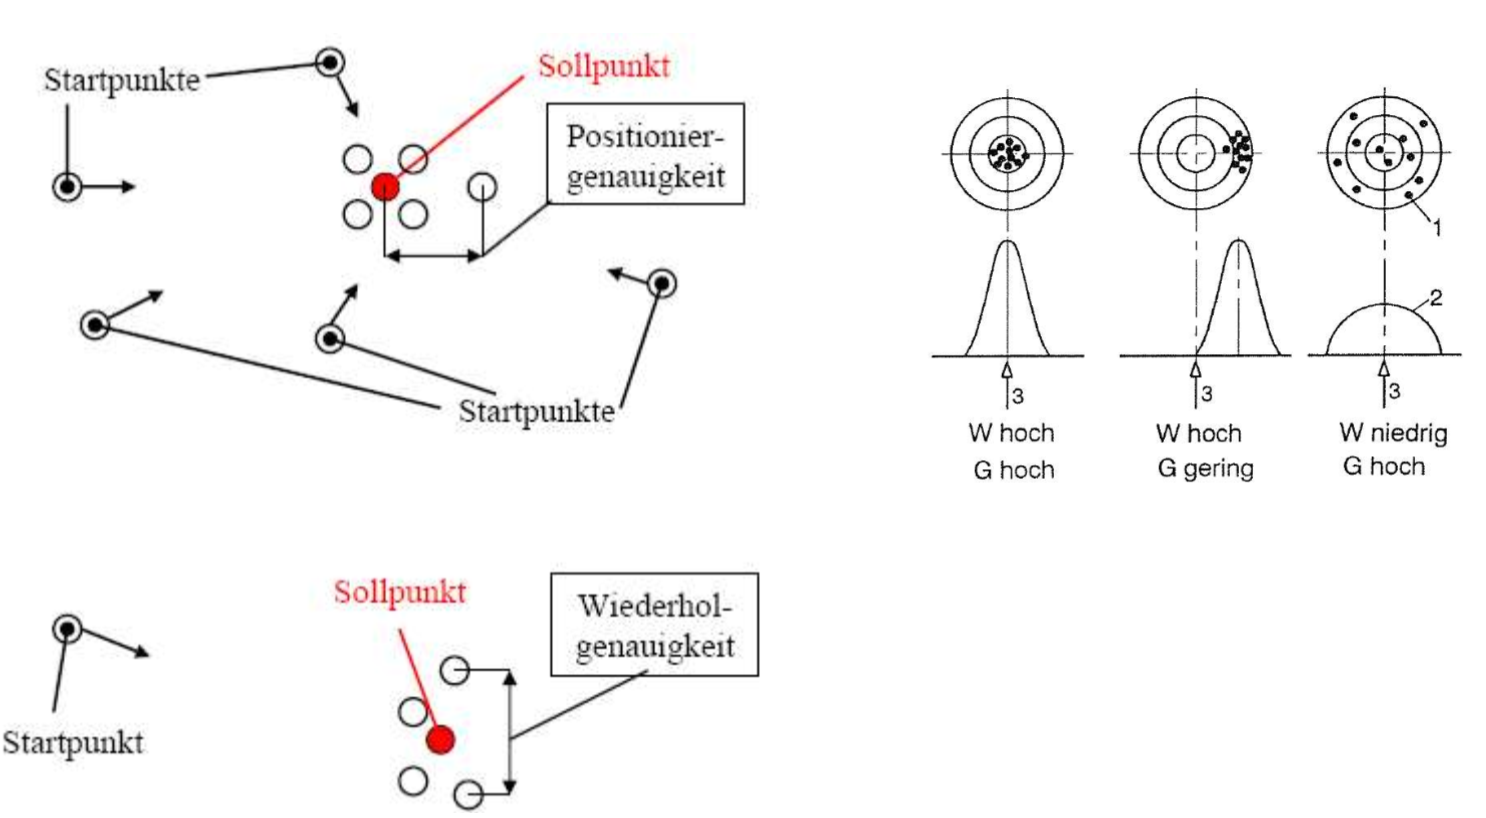
\includegraphics[width=\linewidth]{./bilder/genauigkeit}
\subsection{Anlage}
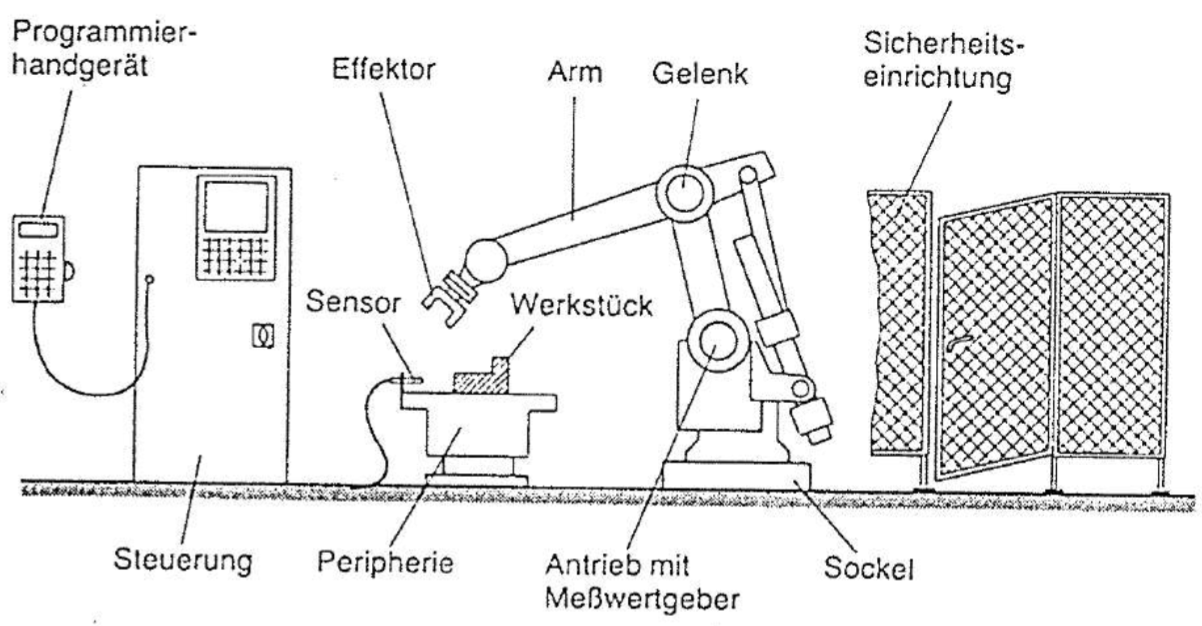
\includegraphics[width=\linewidth]{./bilder/anlage}
\end{minipage}
\begin{minipage}{0.5\linewidth}
\subsection{Anforderungen}
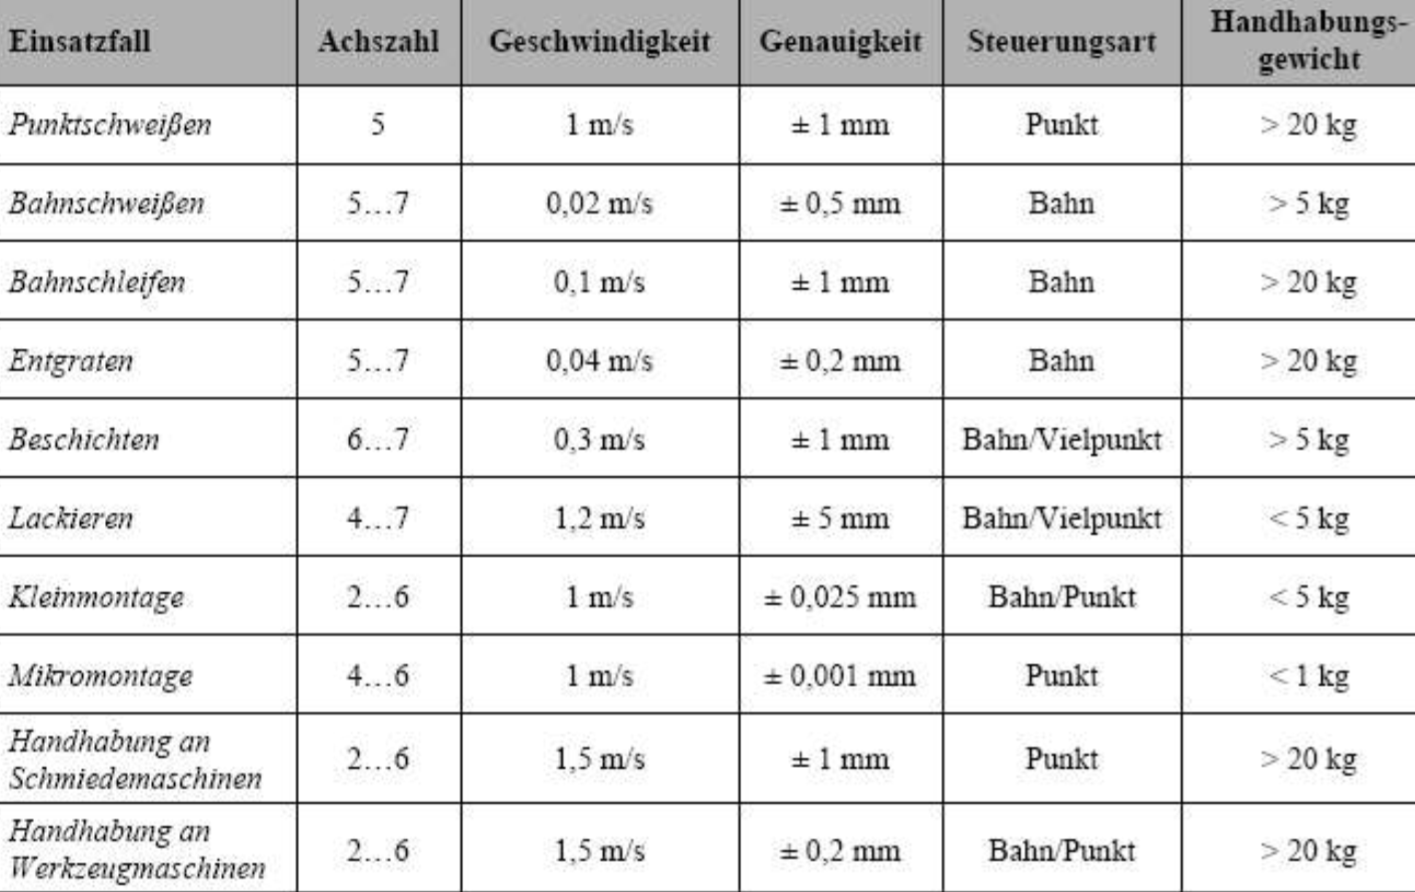
\includegraphics[width=\linewidth]{./bilder/anforderung}
\begin{tabular}{lll}
	\textbf{Art}& \textbf{FG}&\textbf{Grund}\\
	Punktschweissen& 5& Werkzeug rotationssymetrisch\\
	&(6)&(+1 für Kollisionsvermeidung)\\
	Bahnschweissen&6&Schweissen im Raum, Kollisionsvermeidung\\
	Laserschneiden&5&Werkzeug rotationssymetrisch\\
	Palettieren&4&Paletten in einer Ebene, 1 Rotationsachse für Orientierung\\
	Platinen bestücken&4&Platzieren 2, Höhe 1, Orientieren 1\\
	&&\\
\end{tabular}
\end{minipage}

\begin{minipage}{0.5\linewidth}
    \subsection{Komponent}
    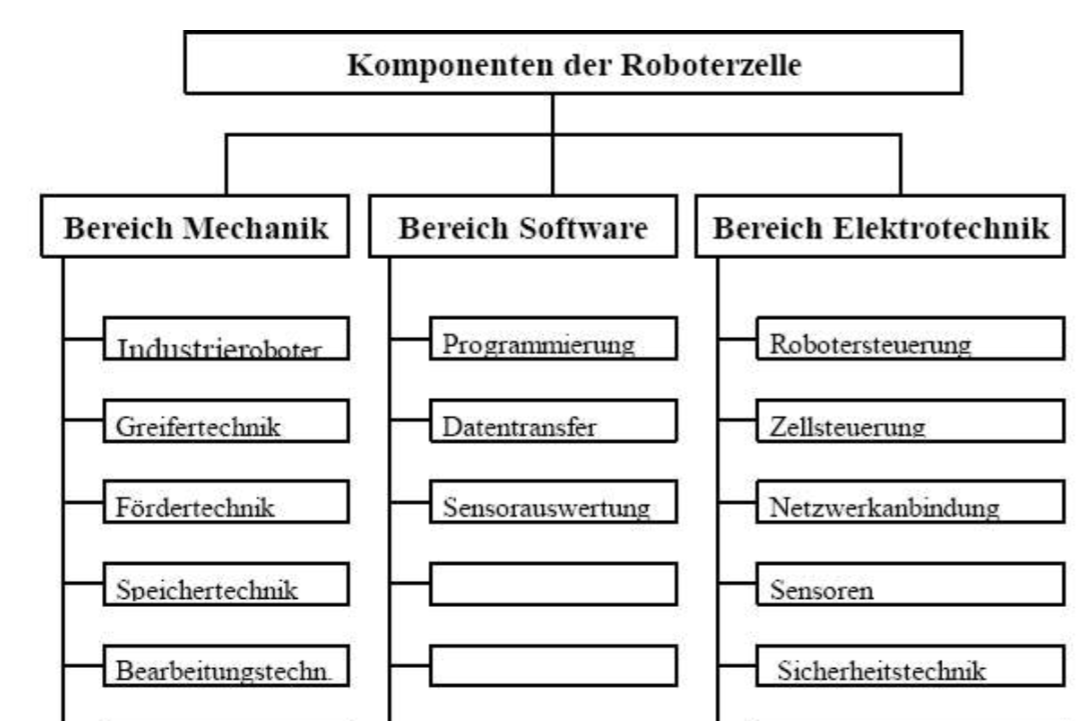
\includegraphics[width=\linewidth]{./bilder/komponent}
\end{minipage}

\begin{minipage}{0.5\linewidth}
\textbf{Es wird empfohlen die Vorlesung 1 auszudrucken}
\end{minipage}

\clearpage
\section{Kinematik}
\subsection{Aufbau}
\begin{minipage}{0.5\linewidth}
\subsubsection{Seriell}
\begin{itemize}
    \item Das erste Armglied ist fest mit dem Boden/Sockel verbunden.
    \item Am letzten Armglied ist ein Effektor befestigt.
    \item An jedem Armgield befindet sich nur ein Gelenk, welches das nächste Armglied verbindet.  
\end{itemize}
\end{minipage}
\begin{minipage}{0.5\linewidth}
\subsubsection{Parallel}
\begin{itemize}
    \item mindestens einen geschlossenen kinematische Kette.
    \item entsteht, wenn ein Armteil auf zwei verschiedenen Wegen mit dem Sockel vebrunden ist.
\end{itemize}
\end{minipage}
	\subsection{Darstellung kinematischer Gelenke}

\begin{minipage}{10cm}
	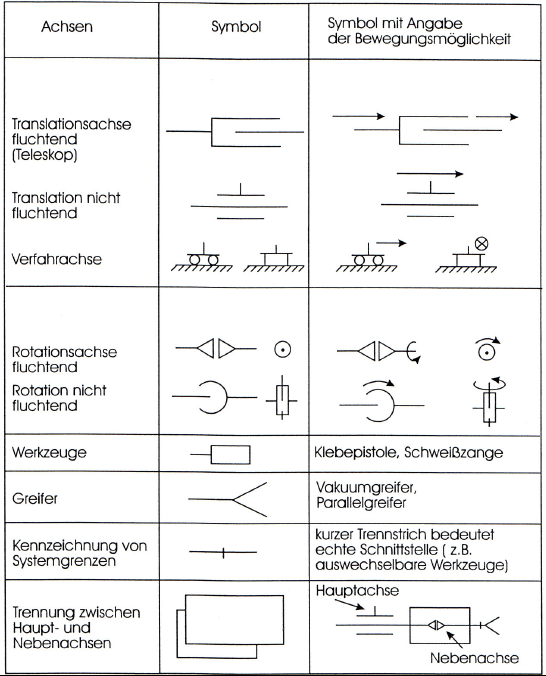
\includegraphics[width=10cm]{./bilder/symbole}
\end{minipage}
\begin{minipage}{8cm}
	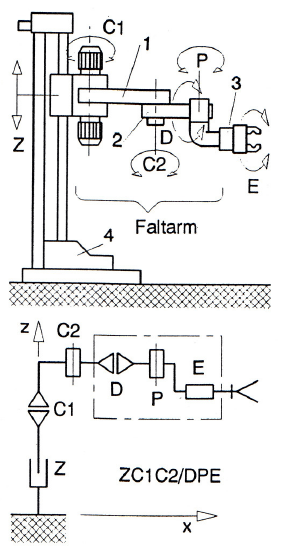
\includegraphics[width=5cm]{./bilder/symbole-bsp}
\end{minipage}



\begin{minipage}{0.5\linewidth}
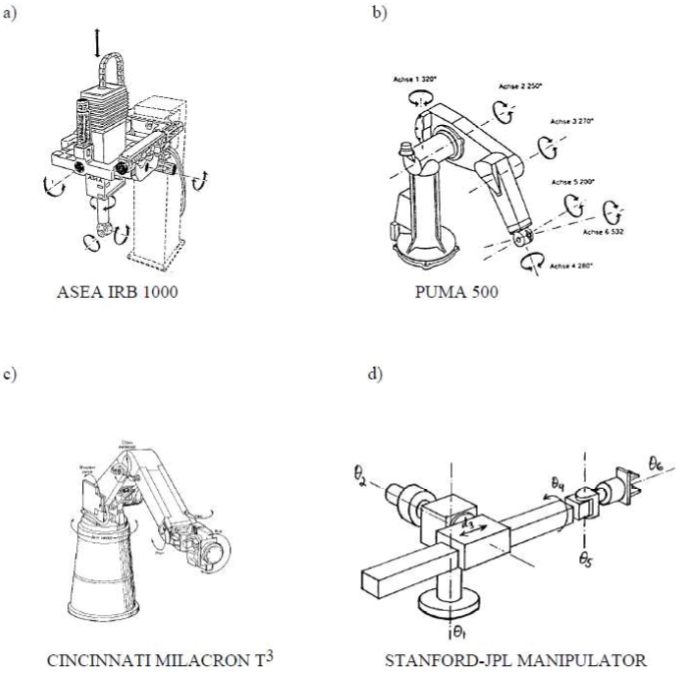
\includegraphics[width=0.8\linewidth]{./bilder/KinAuf}
\end{minipage}
\begin{minipage}{0.5\linewidth}
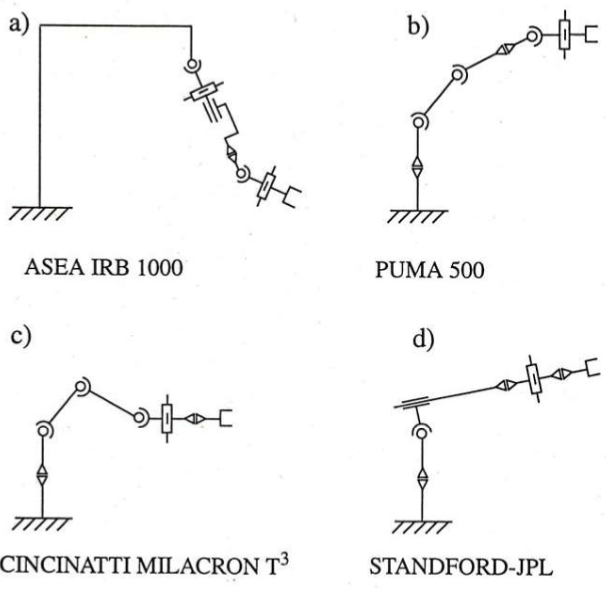
\includegraphics[width=0.8\linewidth]{./bilder/KinAufL}
\end{minipage}



\textbf{TODO Verschiedenen RoboterTypen}